\documentclass[a4paper]{article}

\usepackage[utf8]{inputenc}
\usepackage{microtype}
\usepackage{mathtools, amssymb}
\usepackage{graphicx}
\usepackage{float}

\title{1}
\date{}

\setlength{\parindent}{0em}

\graphicspath{ {../images} }

\begin{document}
\maketitle

\section{ORL Dataset}

The facial recognition system was implemented in \texttt{../code/orl\textunderscore recognition\textunderscore rate.m}.

\medskip
Below is the plot of the recognition rate as a function of $k$:
\begin{figure}[H]
	\centering
	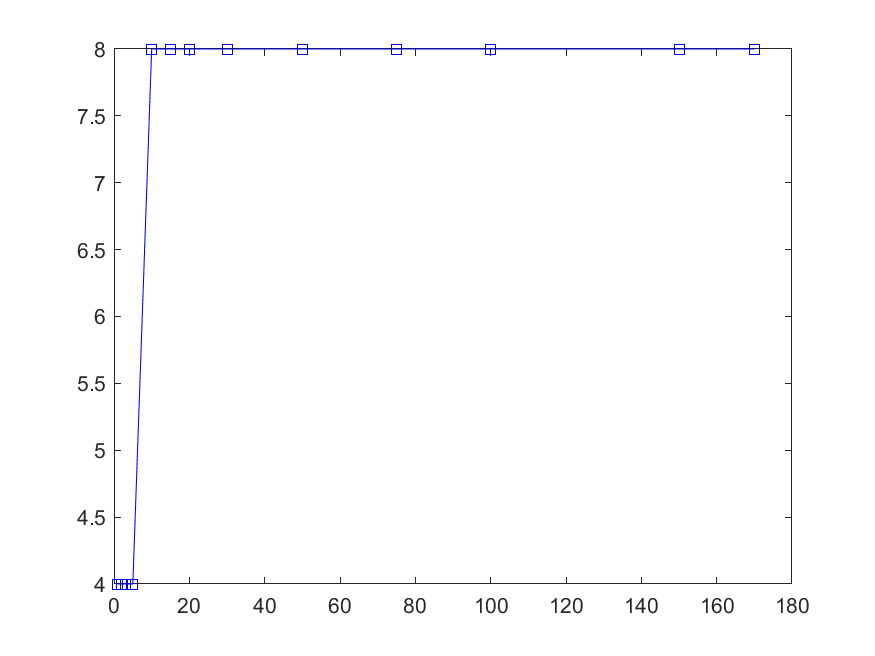
\includegraphics[width=\textwidth]{recognition_rate_orl.png}
	\caption{A plot of the number of faces recognized by the PCA-based facial recognition model as a function of $k$ on the ORL dataset.}
\end{figure}

As can be see in the above image, the facial recognition system consistently recognized 8 faces out of the 32 faces that were in the testing image dataset.

\medskip
The SVD-based implementation of PCA can be found in \texttt{../code/PCA\textunderscore svd.m}.

\section{Yale Dataset}

The plot of the recognition rate as a function of $k$ for the Yale dataset can be found below:
\begin{figure}[H]
	\centering
	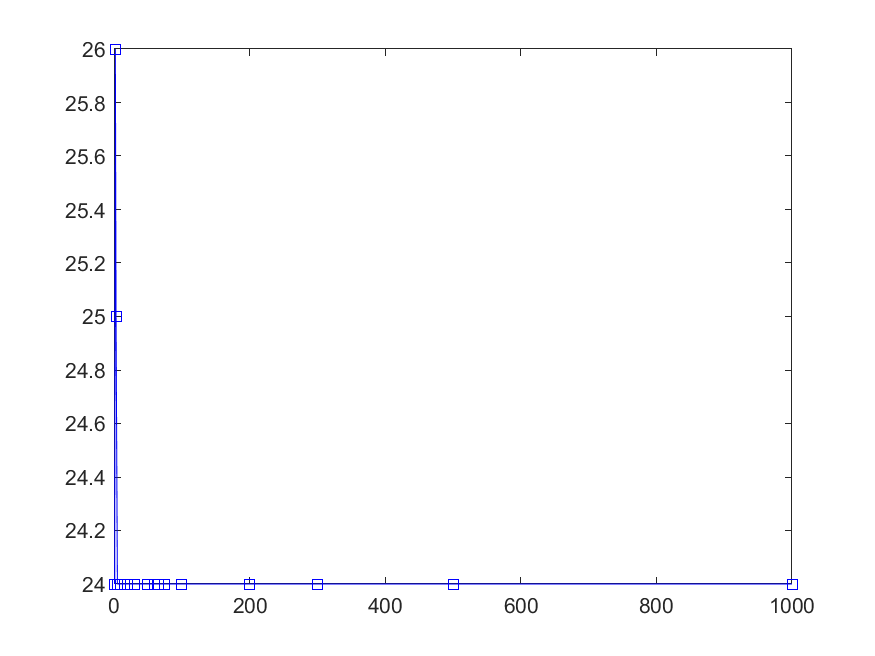
\includegraphics[width=\textwidth]{recognition_rate_yale.png}
	\caption{A plot of the number of faces recognized by the PCA-based facial recognition model as a function of $k$ on the Yale dataset.}
\end{figure}

As can be see in the above image, the facial recognition system consistently recognized between 24 and 26 faces out of the 40 faces that were in the testing image dataset.

\bigskip
If we ignore the three eigencoefficients corresponding to the eigenvectors with the three largest eigenvalues, then the plot becomes slightly different:
\begin{figure}[H]
	\centering
	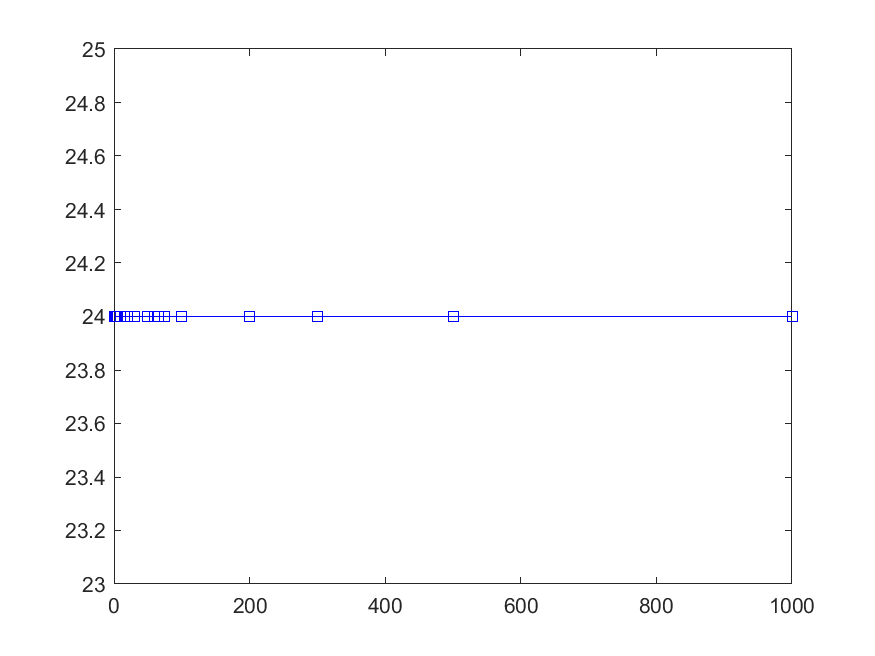
\includegraphics[width=\textwidth]{recognition_rate_yale_partial.png}
	\caption{A plot of the number of faces recognized by the PCA-based facial recognition model as a function of $k$ on the Yale dataset.}
\end{figure}

When we started ignoring the three eigencoefficients corresponding to the eigenvectors with the three largest eigenvalues, the facial recognition system started consistently recognizing precisely 24 out of the 40 faces in the Yale dataset.

\section{Facial Reconstruction using Eigenfaces}

We generated a series of plots of a face reconstructed using eigenfaces, which can be found below:
\begin{figure}[H]
	\centering
	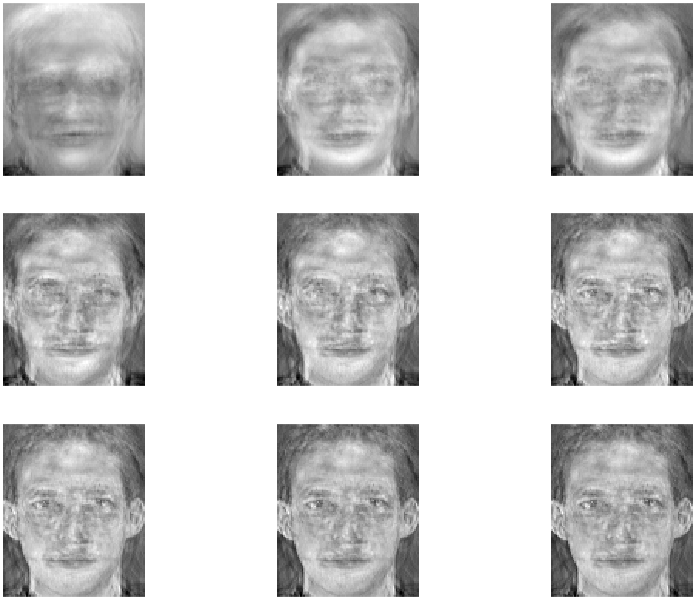
\includegraphics[width=\textwidth]{reconstruction.png}
	\caption{Facial reconstruction using eigenfaces. $k$ is increasing from left to right and top to bottom. $k$ takes values in $\{2, 10, 20, 50, 75, 100, 125, 150, 175\}$ respectively.}
\end{figure}

We used \texttt{../images/ORL/s1/1.pgm} as our test image.

\smallskip
For reference, we decided to add the original image to the report as well:
\begin{figure}[H]
	\centering
	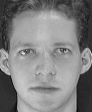
\includegraphics[scale=1]{original.png}
	\caption{The original image, for reference.}
\end{figure}

\newpage
\section{Top 25 Eigenfaces from the ORL Dataset}

Below, we can see the top 25 eigenfaces generated by performing PCA on images in the ORL Dataset.
\begin{figure}[H]
	\centering
	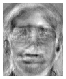
\includegraphics[scale=1]{eigenfaces.png}
	\caption{The top 25 eigenfaces from the ORL dataset.}
\end{figure}

\end{document}